%section{cahier des charges détaillé}

\subsection{Présentation générale du problème}

\subsubsection{Projet}
Le but du sujet est de réaliser un réseau de neurones sur FPGA. Un réseau de neurones est un algorithme schématiquement inspiré du fonctionnement des neurones biologiques. 
On représente un réseau de neurones par un certain nombre de niveau de plusieurs neurones. 
Un neurone est représenté par un noeud qui reçoit des données de la part des neurones du niveau précédent et diffuse sa valeur de sortie aux neurones du niveau suivant. 
Les opérations effectuées sur les données par chaque neurone sont assez simples, se sont des multiplications à accumulations:  $\sum_{i=0}^n w_{i}*d_{i}$, avec $n$ données entrantes dans le réseau, $w_{i}$ le poids pour l'entrée $i$ et $d_{i}$ la données venant du neurones $i$ du niveau précédant. 
Le nombre de niveau et le nombre de neurones sont des paramètres qui peuvent être dimensionnés en fonction de l'application voulu.
Sur la figure~\ref{fig:NN} page~\pageref{fig:NN} vous trouverez un schéma représentant un exemple de réseau de neurones à 3 niveaux.


\begin{figure}[htbp]
\begin{center}
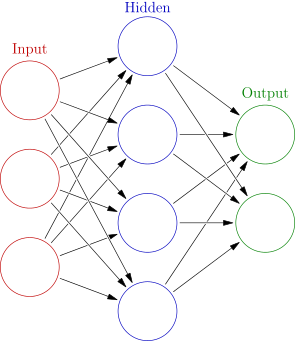
\includegraphics[scale=0.4]{NN}
\caption{Schéma d'un réseau de neurones à 1 niveau "caché" de 4 neurones avec 3 entrées et 2 sorties}
\label{fig:NN}
\end{center}
\end{figure}

\subsubsection{Finalités\\}

Ce réseau de neurones sur FPGA a pour but d'établir une référence pour pouvoir
comparer un réseau de neurones ternaire en cours de développement au laboratoire
TIMA à un réseau de neurones plus classique, tous deux réalisés sur le même 
matériel.

Un objectif secondaire serait de comparer le composant réalisé à d'autres
produits similaires tels que la puce neuromorphique Spinnaker de l'université
de Manchester, ou bien la puce TrueNorth d'IBM.

\subsubsection{Contexte}

Le projet sera réalisé au CIME Nanotech, à Grenoble. 

Quatre heures par semaine sont allouées, dans notre emploi du temps, à la réalisation de ce projet. Cependant,
il est nécessaire de travailler en dehors des horaires prévus pour terminer 
le projet.

Les tests sur carte FPGA seront réalisés dans un premier temps sur une carte Zybo,
puis une fois la fonctionnalité du composant validée, les tests se poursuivront 
sur carte ZedBoard.

\subsubsection{Énoncé du besoin}

Les finalités du produit pour le futur utilisateur tel que prévu par le
demandeur sont:
\begin{itemize}
	\item Il faut concevoir un programme purement logiciel de référence. 
		Celui ci doit respecter les caractéristiques du réseau de neurones demandé, et produire un résultat qui servira de référence à l'IP conçue.
	\item Le composant matériel doit pouvoir être générique, 
		c'est-à-dire qu'il doit être possible de changer le nombre de
		neurones, les coefficients de chaque neurones
		ou encore la taille des données d'entrées, 
		sans la moindre adaptation de code (simplement en changeant les variables voulu dans un fichier).
	\item Le composant matériel doit produire le résultat attendu, c'est-à-dire qu'il
		doit produire un résultat identique au programme de référence.
	\item Le produit étant fortement technique et devant être utilisé par des personnes n'ayant pas conçu cet IP, une documentation détaillée doit être fournie.
\end{itemize}

\subsection{Expression fonctionnelle du besoin}

\subsubsection{Fonctions de service et de contrainte}

\paragraph{Fonctions de service principales\\}
% (qui sont la raison d’être du produit)

Le produit doit calculer le résultat d'une donnée d'entrée soumise à un réseau
de neurones, paramétré selon les coefficients précédemment donnés au composant. 
Dans le cadre de ce projet, les données d'entrée seront les images issues de la base de données MNIST composée d'image de caractères manuscrits. 
Ainsi le but premier du réseau sera de trouver quel caractère lui a été donné en entrée. 

\paragraph{Fonctions de service complémentaires\\}
% (qui améliorent, facilitent ou complètent le service rendu)
Pour une question d'évolution et de réutilisation du projet, le produit rendu doit être reconfigurable très rapidement.
En modifiant seulement quelques variables, le produit doit être capable de s'adapter à d'autres applications que celle prévu pour ce projet.

\paragraph{Contraintes\\}
% (limitations à la liberté du concepteur-réalisateur)

L'architecture globale du composant et ses interfaces (bus, interconnexions, ...) sont déterminées
par le laboratoire TIMA.

Le composant devra utiliser les cellules DSP du FPGA pour réaliser la multiplication à accumulation 
d'un neurone. De plus, il devra utiliser des BRAM pour stocker les coefficients nécessaire aux calculs.

\paragraph{Décomposition en modules, sous-ensembles\\}

L'IP conçue s'intègre dans un environnement complexe. 
Dans un même chip, se trouvent un FPGA, deux coeurs ARM et de nombreuses autres IP tel qu'un DMA, 
de la mémoire et un bus permettant de faire communiquer toutes ces IP entre elles. 
Le réseau de neurones est donc implanté dans le FPGA, et est composé dans l'ordre de propagation des données de :

\begin{itemize}
	\item Une FIFO permettant de récupérer les données envoyées par le micro-processeur via le bus.
	\item Un premier niveau de plus de cents neurones.
	\item Chaque neurone produit un résultat stocké dans une deuxième FIFO.
	\item Les données produites par le premier niveau de neurones passent par une fonction non linéaire.
	\item Ces données ainsi traitées sont envoyées par une FIFO au deuxième et dernier étage de neurones comptant 10 neurones (1 par digit à prédire).
	\item Les résultats finaux sont ainsi renvoyés vers le micro-processeur via le bus AXI du chip.
\end{itemize}
	

\begin{figure}[htbp]
\begin{center}
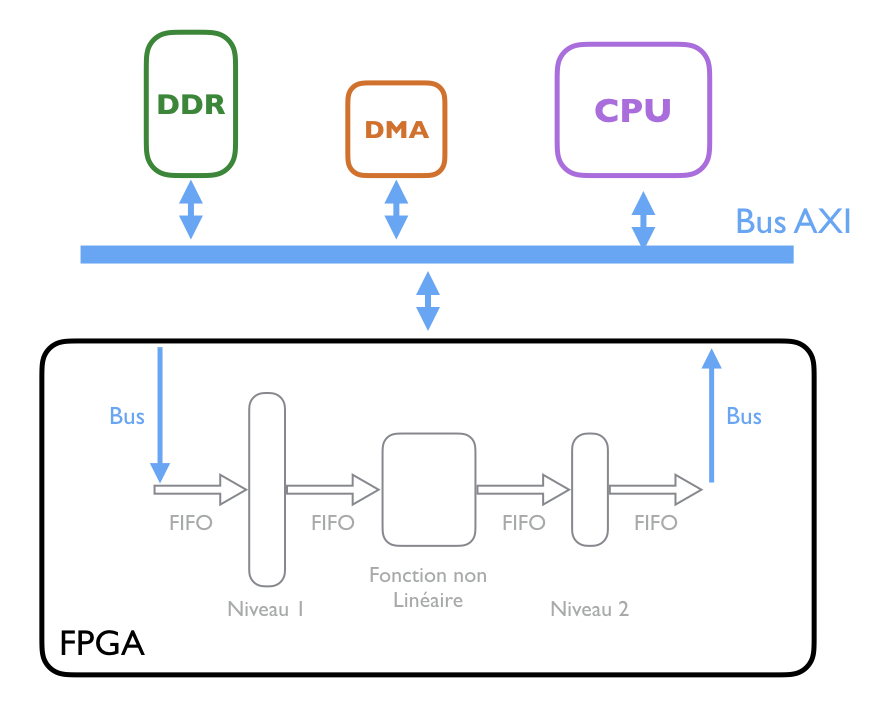
\includegraphics[scale=0.3]{HautNiveauSchema/HautNiveauSchema}
\caption{Schéma haut niveau de l'architecture du réseau de neurones et de son environnement dans le FPGA Xilinx}
\label{fig:NN}
\end{center}
\end{figure}

\subsubsection{Critères d’appréciation}
% (en soulignant ceux qui sont déterminants pour l’évaluation des réponses)

Les critères permettant de mesurer la qualité du composant produit sont:
\begin{itemize}
	\item Correction du composant : le résultat doit être celui attendu.
	\item Taux d'utilisation des cellules du FPGA
	\item Performances du composant (fréquence, nombre de cycles pour
		calculer le résultat ...)
	\item Généricité du composant
\end{itemize}

\subsubsection{Niveaux des critères d’appréciation}
% et ce qui les caractérise

\paragraph{Niveaux dont l’obtention est imposée\\}

Il est nécessaire que le composant satisfasse les niveaux de critères suivants:
\begin{itemize}
	\item Correction : le résultat doit être correct
	\item Taux d'utilisation des cellules du FPGA : un neurone doit utiliser
		une cellule DSP.
\end{itemize}

\paragraph{Niveaux souhaités mais révisables\\}

Il est souhaitable que le composant satisfasse les niveaux de critères suivants:
\begin{itemize}
	\item Performances : Le résultat d'un calcul du composant doit être plus
		rapide que son équivalent réalisé sur un processeur classique.
	\item Généricité : Les fichiers HDL du composant doivent pouvoir être
		modifié de façon mineure pour changer les paramètres du réseau
		de neurones.
\end{itemize}


